% Generated by scripts/generate_article_temporal_sensitivity_outputs.py. Do not edit.
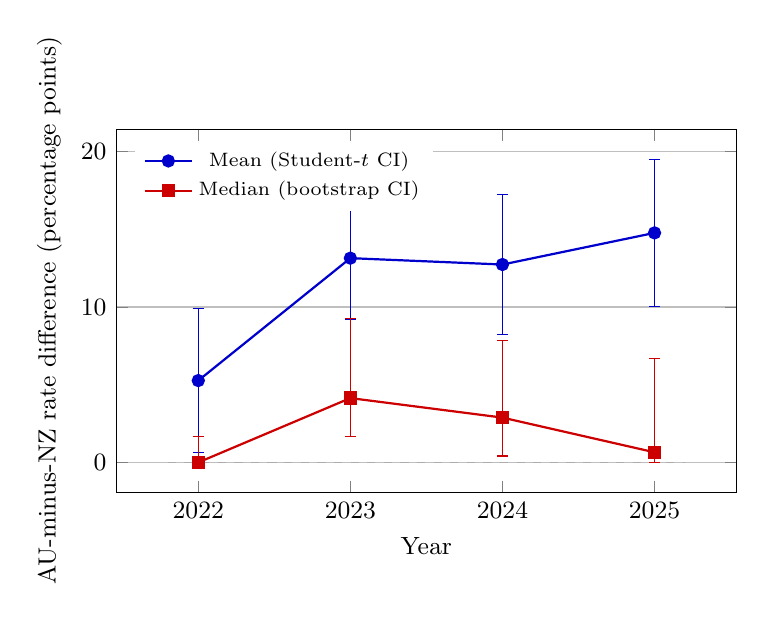
\begin{tikzpicture}
\begin{axis}[width=0.78\textwidth,height=6.2cm,xtick={{2022,2023,2024,2025}},xticklabels={{2022,2023,2024,2025}},xlabel={Year},ylabel={AU-minus-NZ rate difference (percentage points)},ymajorgrids=true,legend style={font=\scriptsize,draw=none,at={{(0.03,0.97)}},anchor=north west},label style={font=\small},tick label style={font=\small}]
\addplot[gray!65,dashed,domain=2021.8:2025.2,forget plot] {0};
\addplot+[blue!80!black,thick,mark=*,error bars/.cd,y dir=both,y explicit] coordinates {(2022,5.26713043495) += (0,4.62154495928) -= (0,4.62154495928) (2023,13.1435706402) += (0,3.92634428999) -= (0,3.92634428999) (2024,12.7334924088) += (0,4.50735861076) -= (0,4.50735861076) (2025,14.7680201261) += (0,4.72986999035) -= (0,4.72986999035)};\addlegendentry{Mean (Student-$t$ CI)}
\addplot+[red!80!black,thick,mark=square*,error bars/.cd,y dir=both,y explicit] coordinates {(2022,0) += (0,1.67301945586) -= (0,0) (2023,4.13992641082) += (0,5.12855217521) -= (0,2.46561913534) (2024,2.88461538462) += (0,4.93555255585) -= (0,2.46918511755) (2025,0.652379260641) += (0,6.04812223288) -= (0,0.652379260641)};\addlegendentry{Median (bootstrap CI)}
\end{axis}
\end{tikzpicture}
